\documentclass[
	parskip=half,10pt,
	numbers= noenddot, % enddot -> Ebenen mit Punkt abschließen -> 1.1., noenddot -> ohne Punkt
	toc=flat, % TOC in Tabellenform (bei langen Überschrtiften verwenden)
	oneside,
	twocolumn,
	]{scrartcl}



\usepackage[T1]{fontenc} % verwende Type 1 - Zeichensatz
\usepackage{libertine}
\usepackage[scaled=0.78]{beramono} %Schreibmaschinenschrift
\usepackage{microtype}
\usepackage[utf8]{inputenc}
\usepackage[english]{babel} % internationale Sprachunterstützung



\usepackage{amsmath}
\usepackage{amssymb}
\usepackage{amsthm}
\usepackage{tabularx}
\usepackage{booktabs}
\usepackage{longtable}
\usepackage{rotating} % Rotationen, Reflexionen, ...
\usepackage{multido} % Wiederholungen
\usepackage{wrapfig}
\usepackage{todonotes}
\usepackage{siunitx} %\si units
\usepackage{units}
\usepackage{icomma} %keine Leerzeichen nach Komma im mathmode
\usepackage[numbers,sort]{natbib}
\usepackage{babelbib} %deutsche bibliographie
\usepackage{multirow}
\usepackage{rotating}
\usepackage{url}

\usepackage{tikz}
\usepackage{float}
\usepackage{pgfplots}
%\pgfplotsset{compat=1.8}
\usepackage{caption}
\usepackage{graphicx}
\usepackage{subcaption} %für subfigures
\captionsetup{labelfont={bf,sf},format = plain, textfont=sf}
%\usepackage{asymptote}
\usepackage{ragged2e}
\usepackage[bottom]{footmisc}
\usepackage{csquotes} %Anführungszeichen
\usepackage[ngerman]{varioref} % Zum komfortablen Verlinken



\usepackage{geometry}
\geometry{a4paper,lmargin=2.5cm, rmargin=2.5cm, tmargin=2.5cm, bmargin=3cm, marginparwidth=3cm, marginparsep=1em}


\usepackage{fancyhdr}
\pagestyle{fancy}
\renewcommand\footrulewidth{0.5pt}
\fancyhf{}
\lhead{\leftmark}

\fancyfoot{}
\rfoot{\thepage}
\lfoot{Till Kolster \& Lukas Schmidt}


\usepackage{layout}

\usepackage[%draft
linkbordercolor=blue,
colorlinks,
linkcolor=blue,
linktocpage,
linktoc=all]{hyperref} % IMMER AM ENDE

%\setkomafont{subparagraph}{\mdseries\itshape}
\setcounter{secnumdepth}{3}%Bis zu welcher Ebene nummeriert werden soll. 
\setcounter{tocdepth}{2}%Bis zu welcher Tiefe ins TOC soll.

%%%%%EIGENE DEFINITIONEN%%%%%

\newcolumntype{Y}{>{\RaggedRight\hspace{0pt}} X }
\newcommand\Grad{$^\circ$}
\newcommand\HAND{\marginnote{\Large\vreflectbox{\ding{43}}}\xspace}%\newcommand\Name{Befehlsdifinition}
\newcommand\MPAR[1]{
\marginnote[\RaggedLeft#1]{\RaggedRight#1}}
% \hspace{0pt} entspricht dem ersten (nicht sichtbaren) Wort
\newcolumntype{P}[1]{>{\RaggedRight\hspace{0pt}}p{#1}}
\newcolumntype{R}{>{\tiny}r}

\pgfmathdeclarefunction{gauss}{4}{%
  \pgfmathparse{#1*exp(-((x-#2)^2)/(2*#3^2))+#4}%
}


\title {Rayleigh-Scattering}
\author {Till Kolster \thanks{Freie Universität Berlin} \and Lukas Schmidt \thanks{Freie Universität Berlin}}


\begin{document}

\begin{titlepage}

\vspace*{-2cm}

\vspace{6cm}
\begin{center}
\huge \bfseries
Fortgeschrittenen-Praktikum -- Rayleigh-Scattering

\vspace{0.5cm}
\large \bfseries
03.12.2014

\vspace{1.5cm}

\large\normalfont von

\bigskip
\textbf{Till Kolster \& Lukas Schmidt}

\bigskip
Tutor: Dr. Andrey Pivtsov

\vspace{3cm}

\parbox{0.8\linewidth}{%
\textit{This experiment is done within the scope of the advanced lab course for Bachelor Students at Freie Universität Berlin.
It should give an experimental introduction to Rayleigh scattering processes, the Scattering-Ring-Down Spectroscopy and should
give a better understanding of Rayleigh scattering phenomenon in nature.
}}


\end{center}
\end{titlepage}


\section{Theoretical Principles}

Rayleigh Scattering is a type of elastic scattering of electromagnetic waves at particles, which are significantly smaller than the wavelength of the photon. 
Rayleigh-scattering can be explained by the Mie-theory, which explains the dependence of the scattering-process from the wavelength. 

If there is a collision of an electromagnetic wave with an atom, the atom will be subject of a change of the electromagnetic field produced by the photon. 
This change will be sinusoidal and hence the atom will resonate. Therefore, the atom can be described as a dipole. 
The electric and magnetic dipole field can be described the following way\cite{griffiths}:
\begin{align}
\vec{E}(\vec{r},t) &= -\frac{\mu_0 p_0 \omega^2}{4 \pi}  \frac{\sin\theta}{r} \cos \left ( \omega \left (t-\frac{r}{c}\right ) \right )\hat{e}_{\theta} \\
\vec{B}(\vec{r},t) &= -\frac{\mu_0 p_0 \omega^2}{4 \pi}  \frac{\sin\theta}{r} \cos \left ( \omega \left (t-\frac{r}{c}\right ) \right )\hat{e}_{\phi},
\end{align}
where $\omega$ is the dipole-frequency and $p_0$ the dipole-moment. 
The probability that a scattering process will take can be described by the scattering cross-section $\sigma$:
\begin{align}
\sigma(\nu) &= \frac{8 }{3} \pi \frac{e^2}{m_e c^2} \frac{\nu^4}{\omega^4},
\end{align}
where $\nu$ is the frequency of the wave. Since (in our case) we have oscillating atoms, $\omega \ll \nu$, because $\lambda \gg$ size of the atom. 
We may replace $\nu= \nicefrac{c}{\lambda}$ to get the dependence of the wavelength. 
In the case of several atoms $N$ and the resulting refraction-index $n$ we can rewrite $\sigma$ as:
\begin{align}
\sigma (\lambda) &= \frac{8 \pi (n^2 -1)^2}{3 N^2 \lambda^4}
\end{align}
With this scattering-cross-section it is easy to get the scattering factor  $\beta$:
\begin{align}
\beta &= N \sigma = \frac{8 \pi (n^2 -1)^2}{3 N \lambda^4}
\end{align}
With the dependence of $\lambda^4$ the colors of the sky can be explained: Taking a sunset or sunrise it can be observed that the sky appears red in the direction of the sun and blue in other directions. This is because sunlight gets scatterd while passing the atmosphere and especially the troposphere. As photons with larger $\lambda$ have a lower cross-section and therefore a lower probability to get scatterd, more of these photons arrive on the direct way from the sun to the earth as their more energetic collegues. These more energetic photons with smaller $\lambda$ have a higher probability to get scatterd and arrive at the observer on the earth especially in the indirect way and turn the sky blue.
\section{Cavity Ring-Down Spectroscopy and Set-Up}

To measure the Rayleigh-scattering, in this experiment a cavity-ring-down-spectrometer ist used. 
\begin{figure}[h]
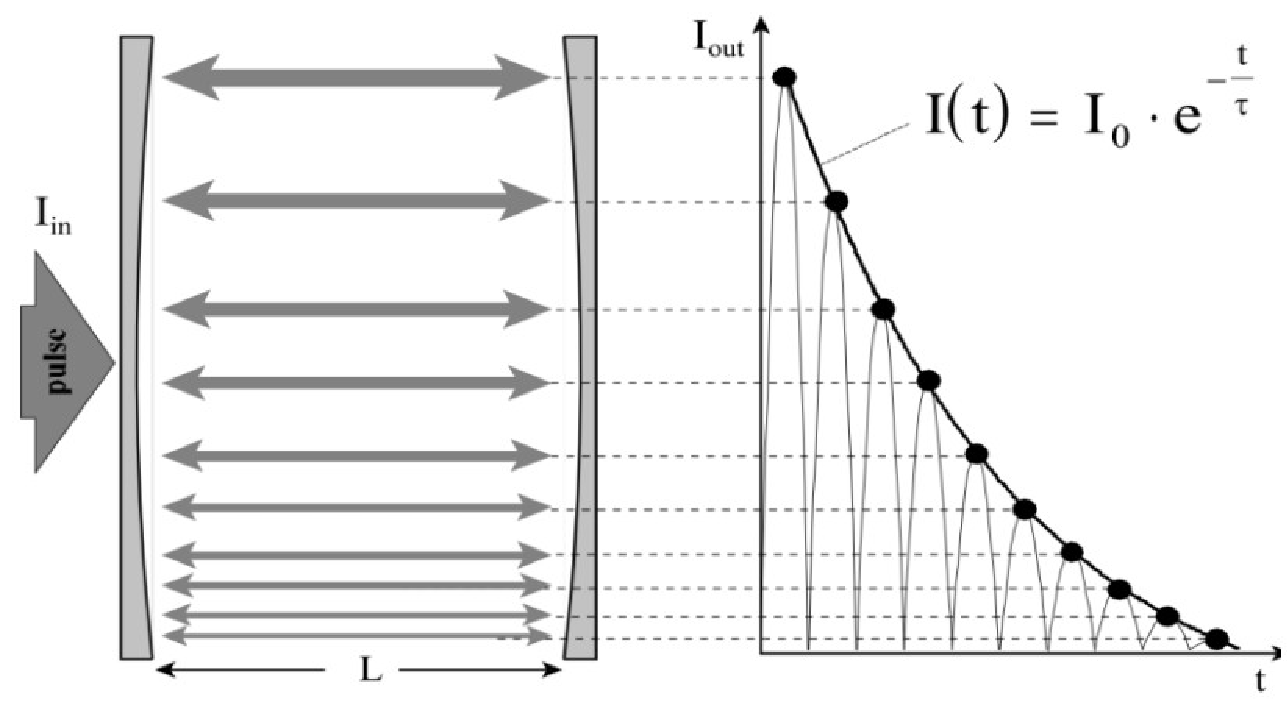
\includegraphics[width=.48 \textwidth]{images/crds.pdf}
\caption{Schematic set-up of a cavity-ring-down-spectrometer \cite{wiki}}
\label{fig:set-up}
\end{figure}
The cavity-ring-down-spectrometer is made of two spherical mirrors and a tube, which can be evacuated. A laser-beam is introduced into the cavity and may be reflected 
several times, to maximize the length of interaction with the medium in the cavity. This way, scattering with a very small number of particles can be measured. 
The reflectance of the mirrors is at about $R=99.98 \%$, so each time the beam hits one of the mirrors about $0.02\%$ of the light is 
transmitted. Behind one of the mirrors is a detector which measures the transmitted part of the beam. The signal intensity $I$ which is recorded this way is 
decreasing exponentially with the time $t$. This is caused by two different mechanisms: Scattering and reflection:
\begin{align}
I(t) &= I_0 e^{-\frac{t}{\tau}}=I_0 e^{- t \left ( \beta c + \frac{1}{\tau_0} \right )},
\end{align}
where $I_0$ is the starting intensity and $\tau_0$ the damping by reflection. It can be expressed the following way:
\begin{align}
\tau_0 &= \frac{L}{c(1-R)},
\end{align}
with $L$ the length of the cavity. This is the damping, when the cavity is evacuated. If a gas is introduced, we get:
\begin{align}
\tau(t) &= \frac{L}{c(1-R(\lambda) + \beta(\lambda)L)}
\end{align}
By comparison of the damping constant in the evacuated and the non-evacuated case, the coefficient $\beta$ can be calculated. 

\begin{figure}[b]
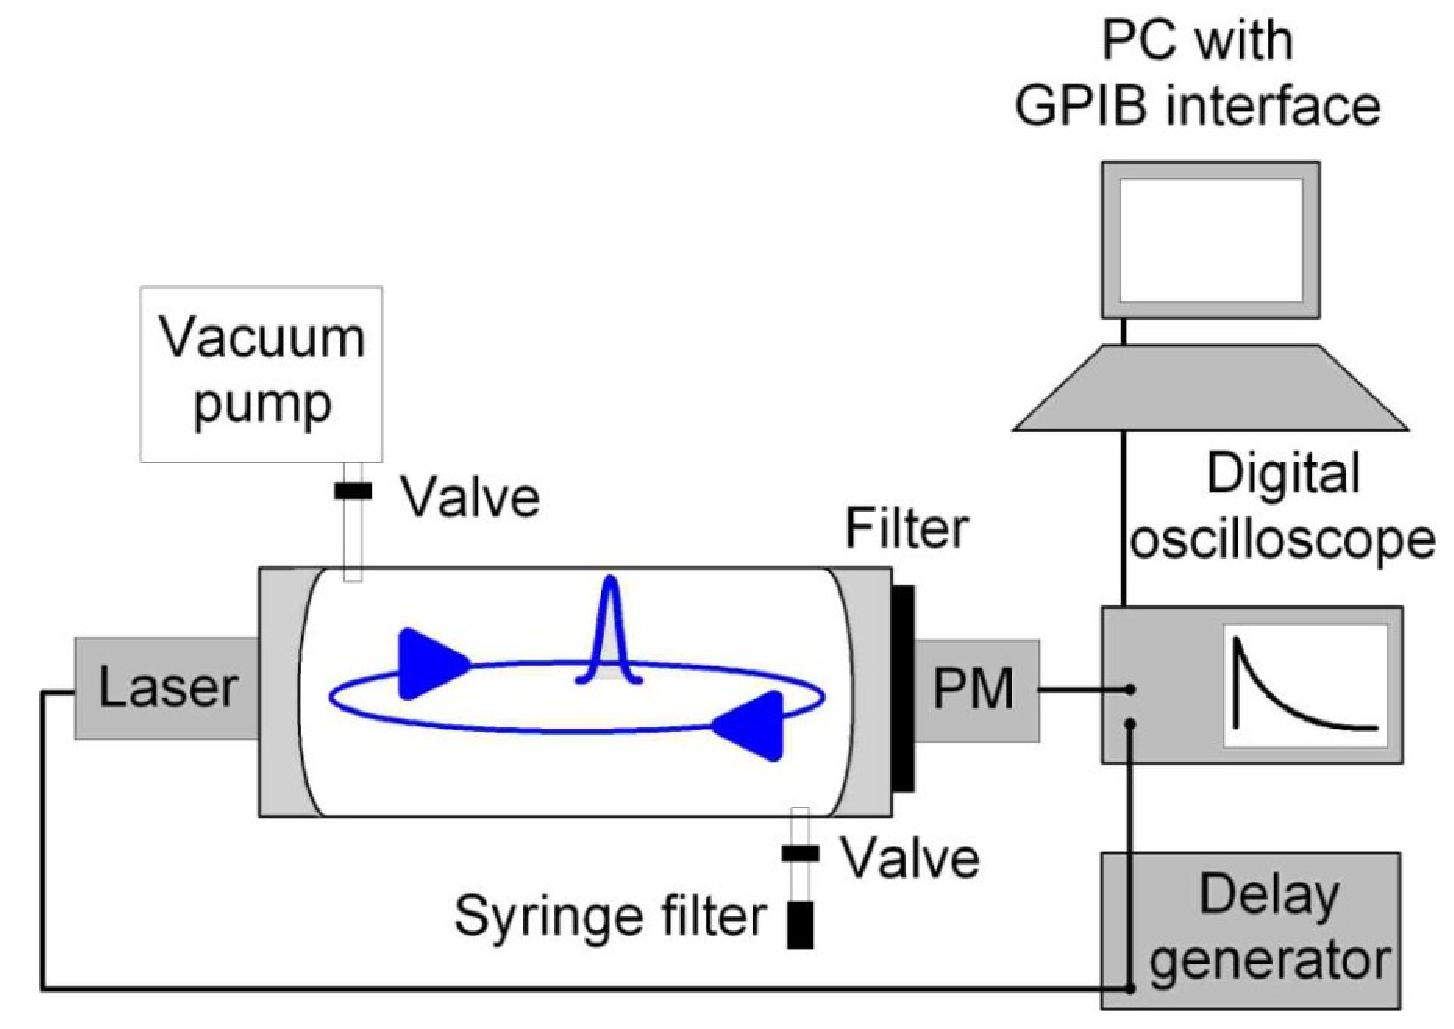
\includegraphics[width = .48 \textwidth]{images/aufbau.pdf}
\caption{Set-up of the experiment \citep{wiki}}
\label{fig:experiment}
\end{figure}

\newpage
\bibliographystyle{unsrtnat}
\bibliography{raybib}

\end{document}





